\section{TBD}

  \subsection[Algebraic Extension of Field R]{Algebraic Extension of Field $\mathbb{R}$}

  We introduce the number $i$, called the \textbf{imaginary unit}, such that $i^2 = -1$. We may multiply real numbers $y$ to $i$ to get $yi$, and we can add real numbers to such numbers, to get numbers of the form 
  \[x + yi, \;\;\; x, y \in \mathbb{R}\]
  We then define all objects of the form $x + iy$ as the \textbf{complex numbers}, with addition defined
  \[(x_1 + i y_1) + (x_2 + i y_2) \equiv (x_1 + x_2) + i (y_1 + y_2)\]
  and multiplication defined
  \[(x_1 + i y_1) \cdot (x_2 + i y_2) \equiv (x_1 x_2 - y_1 y_2) + i (x_1 y_2 + x_2 y_1)\]
  As expected, this makes $+$ and $\cdot$ commutative operations. Furthermore, two complex numbers $z = x_1 + i y_1$ and $w = x_2 + i y_2$ are equal if and only if $x_1 = x_2$ and $y_1 = y_2$. 

  One nontrivial property of field $\mathbb{C}$ is that every element $z \in \mathbb{C}$ has a multiplicative inverse $z^{-1}$. To find this, we must define the following. 

  \begin{definition}[Complex Conjugate]
    Given complex number $z = x + i y$, its \textbf{complex conjugate} is 
    \[\overline{z} = \overline{x + iy} = x - iy\]
    Note that 
    \[z \cdot \overline{z} = x^2 + y^2 \neq 0 \text{ iff } z \neq 0\]
  \end{definition}

  Thus, given $z$, 
  \[z^{-1} = \frac{1}{z \cdot \overline{z}} \cdot \overline{z} \iff (x + yi)^{-1} = \frac{x}{x^2 + y^2} - i \frac{y}{x^2 + y^2}\]

  \subsubsection[Geometric Interpretation of C]{Geometric Interpretation of $\mathbb{C}$}
  Once the algebraic operations $+$ and $\cdot$ has been introduced, the symbol $i$ is no longer needed. That is, we can define a new set $\mathbb{R}^2 = \mathbb{R} \times \mathbb{R}$ with the operations $+_\mathbb{R}, \cdot_\mathbb{R} : \mathbb{R}^2 \times \mathbb{R}^2 \longrightarrow \mathbb{R}^2$ defined
  \begin{align*}
      (x_1, y_1) +_\mathbb{R} (x_2, y_2) & \equiv (x_1 + x_2, y_1 + y_2) \\
      (x_1, y_1) \cdot_\mathbb{R} (x_2, y_2) & \equiv (x_1 x_2 - y_1 y_2, x_1 y_2 + x_2 y_1)
  \end{align*}
  We can check that this new set $(\mathbb{R}^2, +_\mathbb{R}, \cdot_{\mathbb{R}})$ is isomorphic to $(\mathbb{C}, +, \cdot)$ as fields, and therefore one can identify complex numbers with vectors $z = (x, y)$ of the plane $\mathbb{R}^2$, where $x = \text{Re}\,z$ is called the \textbf{real part} and $y = \text{Im}\,z$ is called the \textbf{imaginary part}. 

  \begin{definition}[Norm, Metric of $\mathbb{C}$]
    Moreover, the isomorphism
    \[\gamma: \mathbb{C} \longrightarrow \mathbb{R}^2, \;\; \gamma(x + yi) = (x, y)\]
    induces additional structures on $\mathbb{C}$, such as the norm and metric. 
    \begin{enumerate}
      \item The norm of $z = x + iy \in \mathbb{C}$ is defined as the norm of $\gamma(z) = (x, y) \in \mathbb{R}^2$. That is, 
      \[|z| = |x + yi| = |(x, y)| = \sqrt{x^2 + y^2}\]
      Or more simply, 
      \[|z| = z \cdot \overline{z}\]
      \item The metric of two complex numbers $z_1, z_2 \in \mathbb{C}$ is defined
      \[|z_1 - z_2| = |(x_1, y_1) - (x_2, y_2)| = |(x_1 - x_2, y_1 - y_2)| = \sqrt{(x_1 - x_2)^2 + (y_1 - y_2)^2}\]
      Or more simply, 
      \[|z_1 - z_2| = (z_1 - z_2) \cdot \overline{(z_1 - z_2)}\]
    \end{enumerate}
  \end{definition}

  \begin{definition}[Polar Coordinates of $\mathbb{C}$]
    Given the basis transformation of polar coordinates $(r, \varphi) \mapsto p(r, \varphi) = (x, y)$ where 
    \[p\begin{pmatrix} r \\ \varphi \end{pmatrix} = \begin{pmatrix}
    r \cos{\varphi} \\ r \sin{\varphi} 
    \end{pmatrix} = \begin{pmatrix} x \\ y \end{pmatrix}\]
    the isomorphism $\mathbb{C} \simeq \mathbb{R}^2$ induces a similar polar transformation in $\mathbb{C}$
    \[\rho = \gamma^{-1} \circ p \circ \gamma: \mathbb{C}_{(r, \theta)} \longrightarrow \mathbb{C}_{(x, y)}, \;\;\rho(r + \theta i) = r \cos{\theta} + r \sin{\theta} i = x + y i\]
    as shown in the commutative diagram. 
    \[\begin{tikzcd}
        \mathbb{C}_{(r, \theta)} \arrow{d}{\gamma} \arrow{r}{\rho} & \mathbb{C}_{(x, y)} \arrow{d}{\gamma} \\
        \mathbb{R}^2_{(r, \theta)} \arrow{r}{p} & \mathbb{R}^2_{(x, y)}
      \end{tikzcd}\]
    Therefore, we can write 
    \[z = r ( \cos{\varphi} + i \sin{\varphi})\]
    where $r = |z|$ is called the \textbf{magnitude} of $z$, and $\varphi = \text{Arg}\,z$ is called the \textbf{argument} of $z$. 
  \end{definition}

  \begin{lemma}[Multiplication of Complex Numbers in Polar Form]
    It turns out that multiplication is a lot easier in polar coordinates than in rectangular ones: 
    \begin{align*}
        z_1 \cdot z_2 & = (r_1 \cos{\varphi_1} + i r_1 \sin{\varphi_1})(r_2 \cos{\varphi_2} + i r_2 \sin{\varphi_2}) \\
        & = \ldots \\
        & = r_1 r_2 \big(\cos{(\varphi_1 + \varphi_2)} + i \sin{(\varphi_1 + \varphi_2)}
    \end{align*}
    \begin{center}
        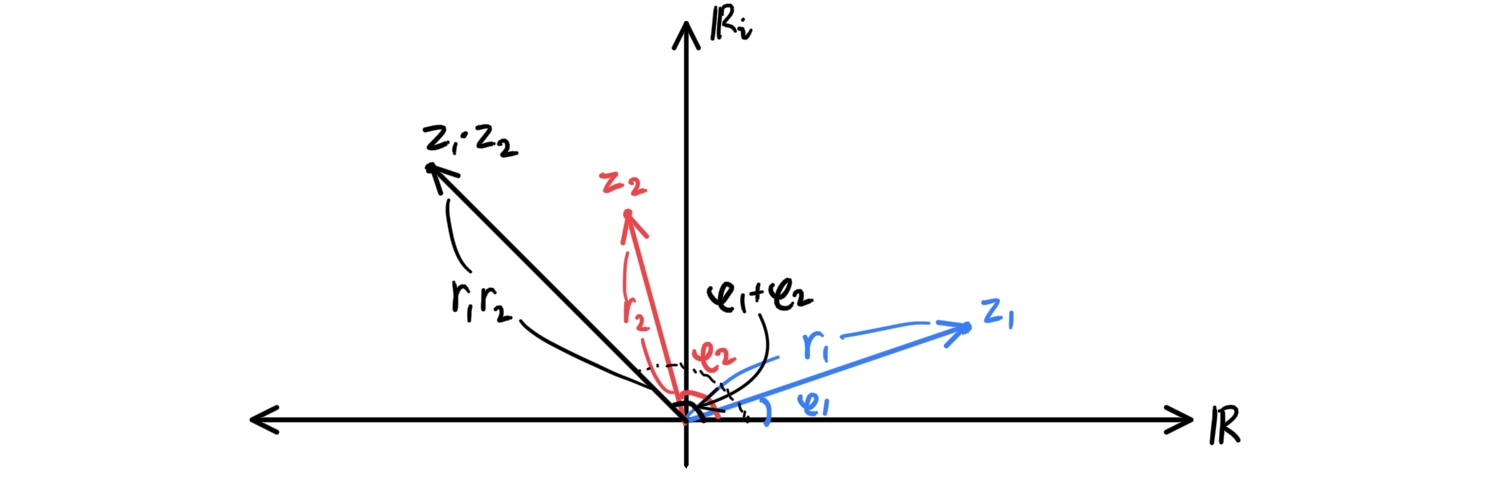
\includegraphics[scale=0.25]{img/Multiplication_Complex_Polar_Form.jpg}
    \end{center}
  \end{lemma}

  \begin{theorem}[De Moivre's Formula]
  By induction using the previous lemma, we get 
  \[z = r ( \cos{\varphi} + i \sin{\varphi}) \implies z^n = r^n (\cos{n\varphi} + i \sin{n \varphi})\]
  \end{theorem}

  \begin{corollary}[Roots of Unity]
  The $n$ complex solutions of the equation 
  \[z^n = a\]
  where $a = \rho (\cos{\psi} + i \sin{\psi})$ is 
  \[z_k = \sqrt[n]{\rho} \bigg( \cos\Big(\frac{\psi + 2\pi k}{n} \Big) + i \sin\Big(\frac{\psi + 2\pi k}{n}\Big) \bigg), \;\;\;\;\; k = 0, 1, 2, \ldots, n-1\]
  Moreover, if $a = 1$, then the $n$ complex solutions are called the \textbf{$n$th roots of unity}, defined
  \[z_k = \cos\Big(\frac{2\pi k}{n}\Big) + i \sin\Big(\frac{2\pi k}{n}\Big), \;\;\;\;\; k = 0, 1, 2, \ldots, n-1\]
  which shows that the $n$th roots of unity are at the vertices of a regular $n$-sided polygon inscribed in the unit circle, with one vertex at $1$, within the complex plane. The $5$th and $6$th roots of unity are shown below. 
  \begin{center}
      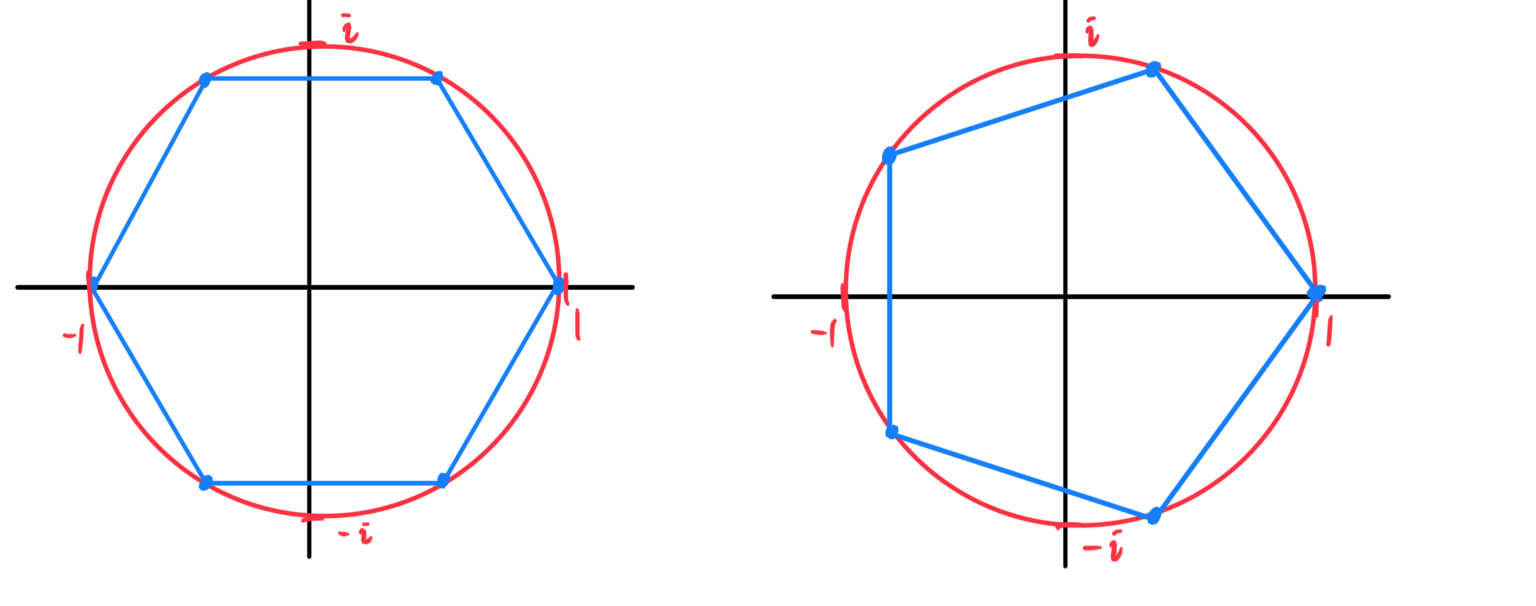
\includegraphics[scale=0.27]{img/5th_6th_Roots_of_Unity.PNG}
  \end{center}
  \end{corollary}

  Finally, we can visualize certain transformations in $\mathbb{C}$. For a fixed $b \in \mathbb{C}$, the sum $z + b$ cam be interpreted as the mapping of $\mathbb{C}$ onto itself given by the formula 
  \[z \mapsto z + b\]
  This mapping is a translation of the plane by the vector $b$. 
  \begin{center}
      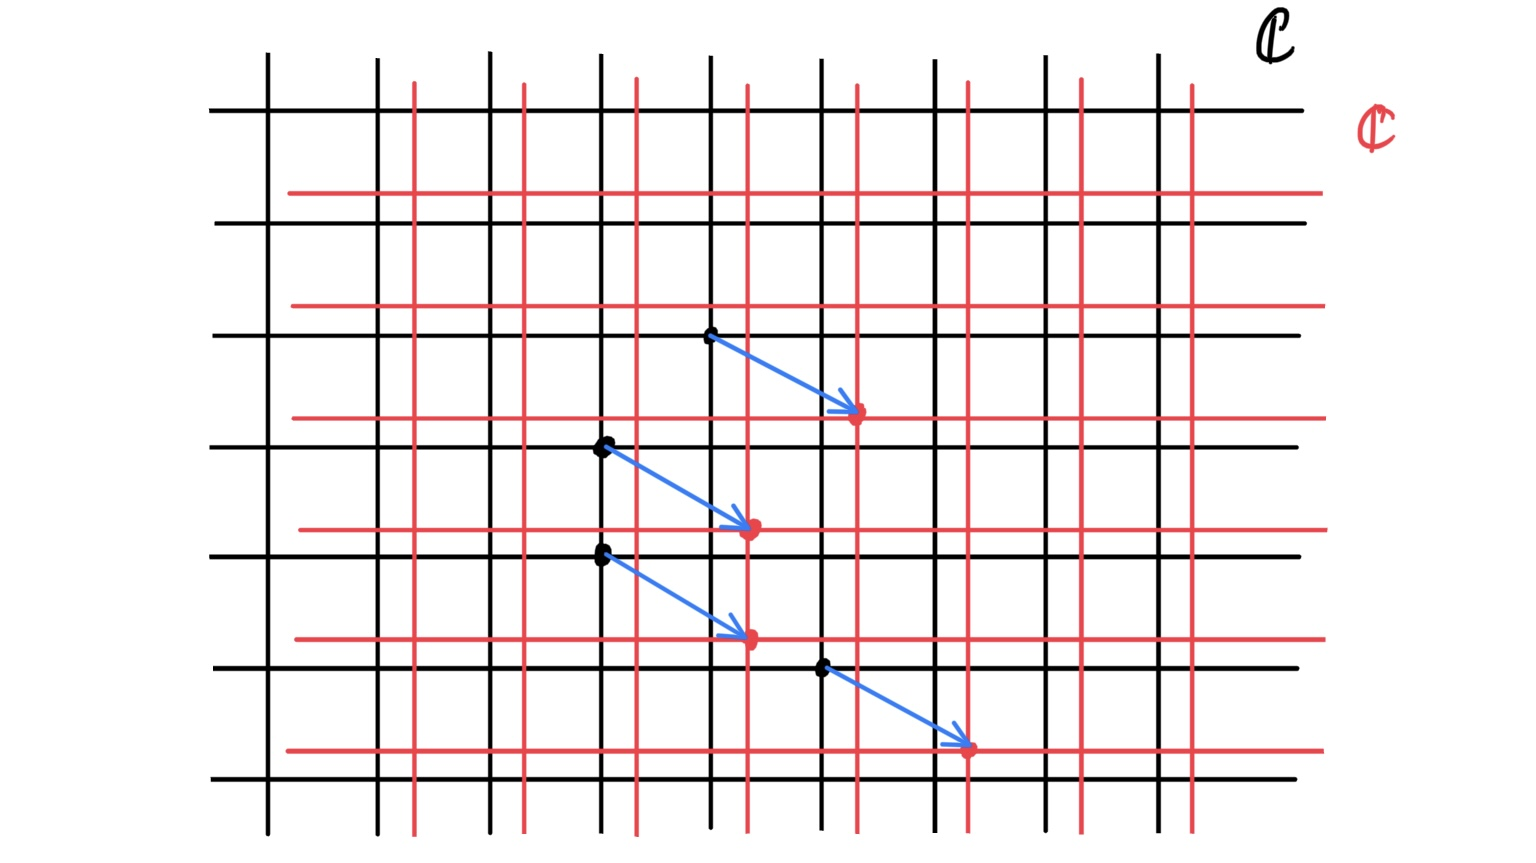
\includegraphics[scale=0.25]{img/Translation_in_Complex_Plane.jpg}
  \end{center}
  Visualizing multiplication is a bit harder. Given a 
  \[a = |a| (\cos{\varphi} + i \sin{\varphi}) \neq 0\]
  the product $az$ can be interpreted as the mapping of $\mathbb{C}$ onto itself given by the formula
  \[z \mapsto az\]
  which is the composition of a dilation by a factor of $|a|$ and a rotation through the angle $\varphi \in \text{Arg}\,a$. 
  \begin{center}
      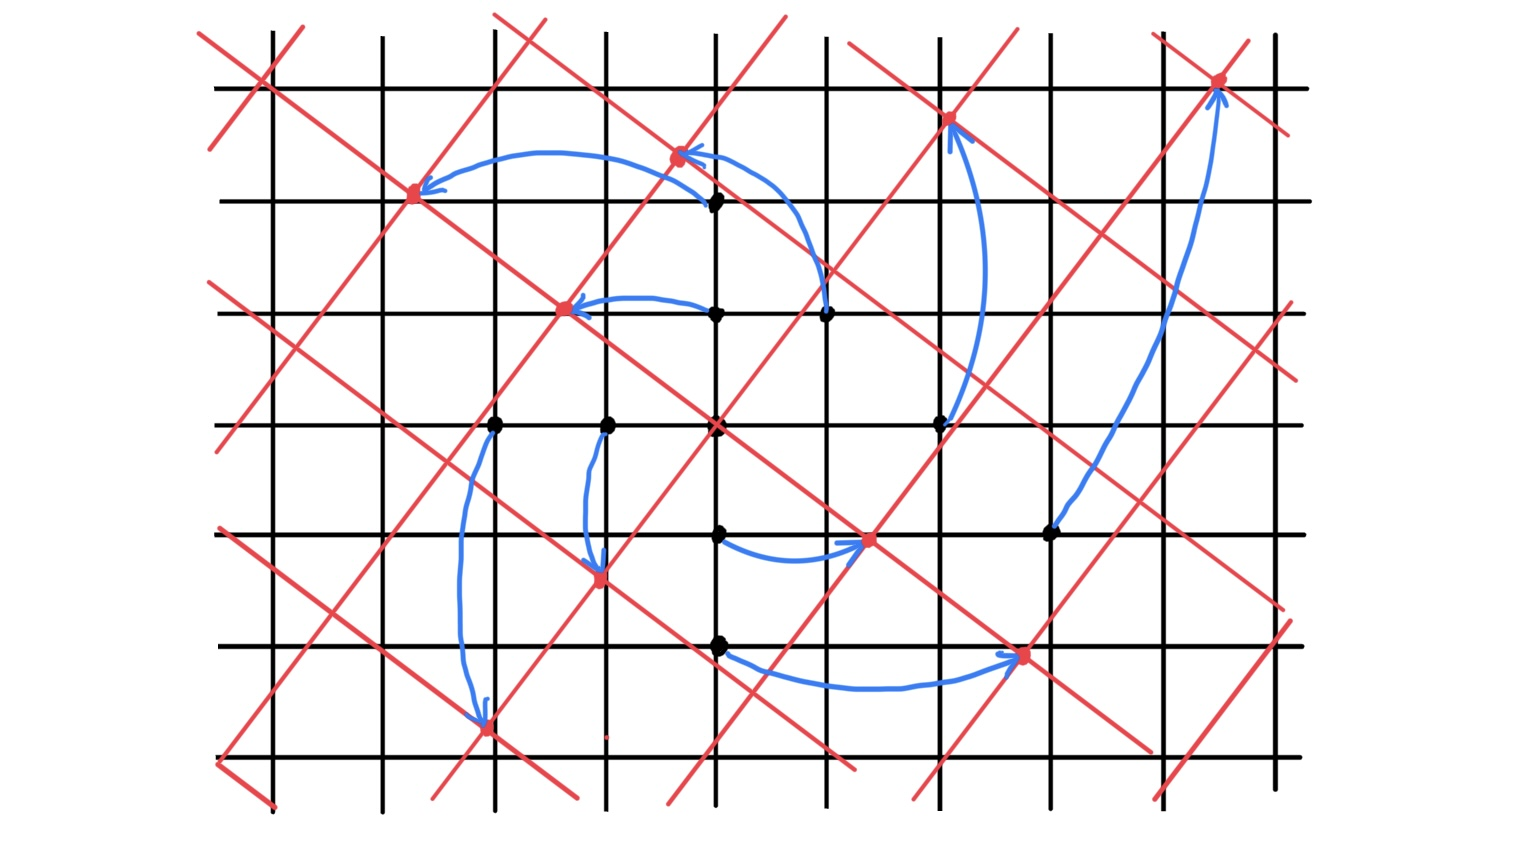
\includegraphics[scale=0.3]{img/Multiplication_in_Complex_Plane.jpg}
  \end{center}

  \subsection[Sequences and Series in C]{Sequences and Series in $\mathbb{C}$}

  Our previous construction of a metric within $\mathbb{C}$ enables to define the $\epsilon$-neighborhood of a number $z_0 \in \mathbb{C}$ as the set
  \[U_\epsilon (z_0) \equiv \{z \in \mathbb{C}\;|\; |z - z_0| < \epsilon\}\]
  which can be visualized as an open disk of radius $\epsilon$ in $\mathbb{R}^2$ centered at point $(x_0, y_0)$ if $z_0 = x_0 + i y_0$. 
  \begin{center}
      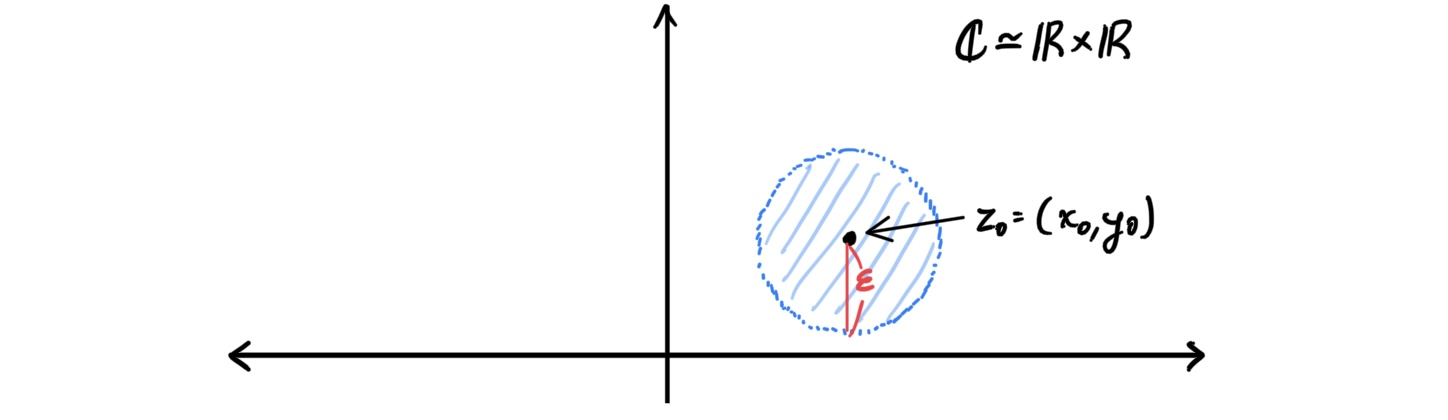
\includegraphics[scale=0.25]{img/Epsilon_Neighborhood_in_C.jpg}
  \end{center}

  \begin{definition}[Convergence of a Sequence in $\mathbb{C}$]
    A sequence $\{z_n\}$ of complex numbers \textbf{converges} to $z_0 \in \mathbb{C}$ if and only if 
    \[\lim_{n \rightarrow \infty} |z_n - z_0| = 0\]
    It is clear from the inequality
    \[\max\{|x_n - x_0|, |y_n - y_0|\} \leq |z_n - z_0| \leq |x_n - x_0| + |y_n - y_0|\]
    that a sequence of complex numbers converges if and only if the sequences of its real and imaginary parts of the terms of the sequence both converge. That is, 
    \[\{z_n\} \text{ converges} \iff \{\text{Re}\,z\} \text{ and } \{\text{Im}\,z\} \text{ converges}\]
  \end{definition}

  \begin{lemma}[Convergence of Cauchy Sequences over $\mathbb{C}$]
    A sequence of complex numbers $\{z_n\}$ is called a \textbf{Cauchy sequence} if for every $\epsilon>0$ there exists an index $N \in \mathbb{N}$ such that
    \[|z_n - z_m|<\epsilon \text{ for all } n, m > N\]
    It is also clear that 
    \[\{z_n\} \text{ is Cauchy} \iff \{\text{Re}\,z\} \text{ and } \{\text{Im}\,z\} \text{ is Cauchy}\]
    and using the Cauchy criterion for sequences of real numbers, we can easily see that a sequence of complex numbers converges if and only if it is a Cauchy sequence. 
  \end{lemma}

  \begin{lemma}[Convergence of Cauchy Series over $\mathbb{C}$]
    Interpreting the sum of a series of complex numbers
    \[z_1 + z_2 + \ldots + z_n + \ldots\]
    as the limit of the sequence its partial sums $\{s_n\}$, where $s_n = z_1 + \ldots z_n$ as $n \rightarrow \infty$, we can see that the series converges if and only if for every $\epsilon > 0$ there exists a $N \in \mathbb{N}$ such that 
    \[|z_m + \ldots + z_n| < \epsilon\]
    for any natural numbers $n \geq m > N$. 
  \end{lemma}

  \begin{definition}[Absolute Convergence of $\mathbb{C}$]
    A series $z_1 + \ldots + z_n + \ldots$ of complex numbers is \textbf{absolutely convergent} if the series
    \[|z_1| + |z_2| + \ldots + |z_n| + \ldots\]
    converges. Clearly, is a series converges absolutely, then it converges due to the inequality
    \[|z_m + \ldots + z_n| \leq |z_m| + \ldots + |z_n|\]
  \end{definition}

  \begin{example}
    The following complex series converges because they converges absolutely. That is, 
    \begin{align*}
        1 + \frac{1}{1!}|z| + \frac{1}{2!}|z^2| + \ldots \text{ converges } \forall \; \mathbb{C} & \implies 1 + \frac{1}{1!}z + \frac{1}{2!}z^2 + \ldots \text{ converges } \forall \; \mathbb{C} \\
        |z| + \frac{1}{3!}|z|^3 + \frac{1}{5!}|z|^5 + \ldots \text{ converges } \forall \; \mathbb{C}  & \implies z - \frac{1}{3!} z^3 + \frac{1}{5!}z^5 + \ldots \text{ converges } \forall \; \mathbb{C} \\
        1 + \frac{1}{2!}|z|^2 + \frac{1}{4!} |z|^4 + \ldots \text{ converges }  \forall \; \mathbb{C} & \implies 1 - \frac{1}{2!}z^2 + \frac{1}{4!} z^4 - \ldots \text{ converges }  \forall \; \mathbb{C} 
    \end{align*}
  \end{example}

  \begin{definition}[Complex Power Series]
    Series of the form 
    \[\sum_{n=0}^\infty c_n (z - z_0)^n = c_0 + c_1 (z - z_0) + \ldots + c_n (z - z_0) + \ldots\]
    are called \textbf{complex power series}, or \textbf{power series over $\mathbb{C}$}. 
  \end{definition}

  But a power series is quite useless unless we know the domain in which is converges (again, note that it is not always guaranteed to converge onto the function $f$ if its power series expansion does converge at all). To develop more sophisticated tests of convergence of a complex power series, we introduce the complex analogue of the root test for real power series. 

  \begin{theorem}[Cauchy-Hadamard Theorem]
  The complex power series 
  \[c_0 + c_1 (z - z_0) + \ldots + c_n (z - z_0) + \ldots\]
  converges inside the disk $|z - z_0| < R$ with center at $z_0$ and radius given by the formula
  \[R = \frac{1}{\varlimsup_{n \rightarrow \infty} \sqrt[n]{|c_n|}} = \frac{1}{\lim_{n \rightarrow \infty} \sup{\sqrt[n]{|c_n|}}}\]
  Where $\varlimsup$ denotes the superior limit. Furthermore, 
  \begin{enumerate}
    \item the power series diverges at any point exterior to the disk. 
    \item the power series converges absolutely at any point interior to the disk. 
    \item the power series is indeterminate at any point on the boundary of the disk. 
  \end{enumerate}
  Note that in the degenerate case when $R = 0$, the series converges only at the point $z = z_0$. 
  \end{theorem}

  \begin{corollary}[Abel's First Theorem on Power Series]
  If the power series 
  \[c_0 + c_1 (z - z_0) + \ldots + c_n (z - z_0) + \ldots\]
  converges at some value $z^*$, then it converges absolutely for any value of $z$ satisfying
  \[|z - z_0| < |z^* - z_0|\]
  The values of $z$ satisfying the inequality above can be intuitively visualized as the following region. 
  \begin{center}
      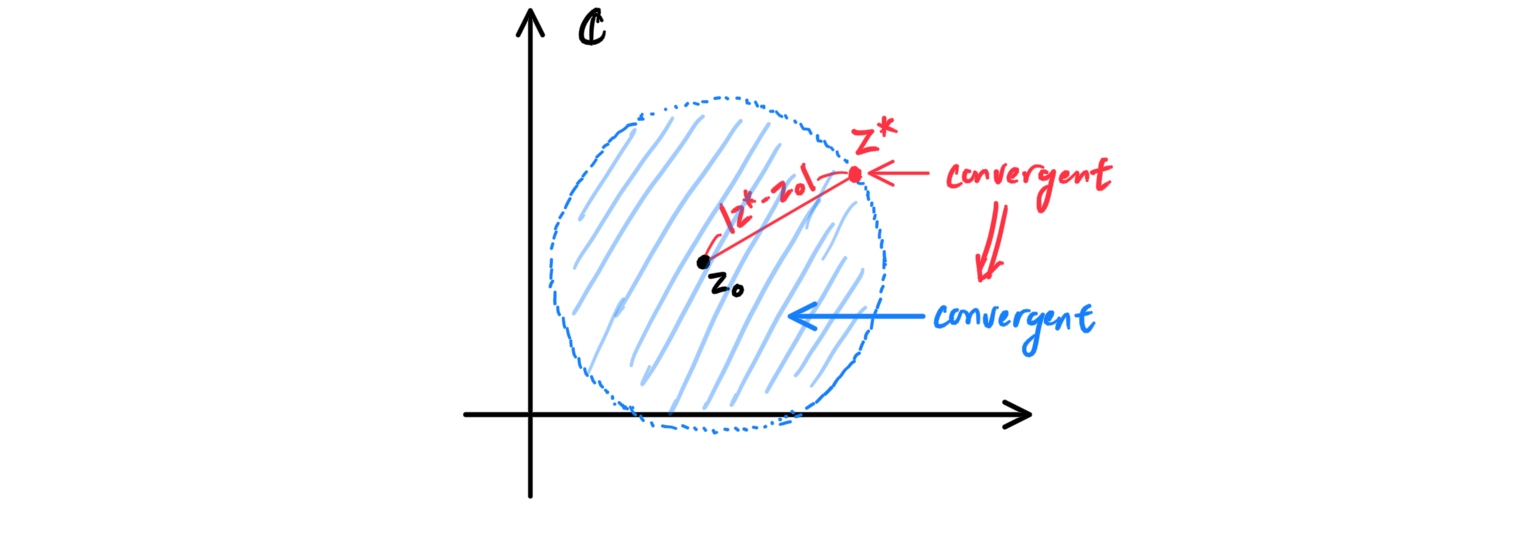
\includegraphics[scale=0.25]{img/Abels_First_Theorem.PNG}
  \end{center}
  \end{corollary}

  \begin{theorem}[Product of Absolutely Convergent Series]
  Let $a_1 + a_2 + \ldots$ and $b_1 + b_2 + \ldots$ be an absolutely convergent series such that
  \[\sum_{i=1}^\infty a_i = A \text{ and } \sum_{j=1}^\infty b_j = B\]
  Then, the Cauchy product of the two series 
  \[\bigg( \sum_{i=1}^\infty a_i \bigg) \cdot \bigg( \sum_{j=1}^\infty b_j \bigg) = \sum_{k=0}^\infty c_k = A B, \text{ where } c_k = \sum_{l=0}^k a_l b_{k-l}\]

  $a_1 b_1 + a_2 b_2 + \ldots$ is absolutely convergent and 
  \[\sum_{i = 1}^\infty a_i b_i = A B\]
  \end{theorem}
  \begin{proof}
  To be done. 
  \end{proof}

    \begin{example}[Convergence of the Cauchy Product of Absolutely Convergent Complex Series]
    The two series 
    \[\sum_{n = 0}^\infty \frac{1}{n!} a^n \text{ and } \sum_{m = 0}^\infty \frac{1}{m!} b^m\]
    converges absolutely. Therefore, we can see that their Cauchy product can be nicely represented by grouping together all monomials of the form $a^n b^m$ having the same total degree $m + n = k$. 
    \[\bigg( \sum_{n = 0}^\infty \frac{1}{n!} a^n \bigg) \cdot \bigg( \sum_{m = 0}^\infty \frac{1}{m!} b^m \bigg) = \sum_{k=0}^\infty \bigg(\sum_{n+m=k} \frac{1}{n!} a^n \frac{1}{m!} b^m \bigg)\]
    But we can simplify 
    \[\sum_{m + n = k} \frac{1}{n! m!} a^n b^m = \frac{1}{k!} \sum_{n=0}^k \frac{k!}{n! (k-n)!} a^n b^{k-n} = \frac{1}{k!} (a + b)^k\]
    and therefore we find that 
    \[\bigg( \sum_{n = 0}^\infty \frac{1}{n!} a^n \bigg) \cdot \bigg( \sum_{m = 0}^\infty \frac{1}{m!} b^m \bigg) = \sum_{k=0}^\infty \frac{1}{k!} (a + b)^k\]
  \end{example}

    \subsection{Euler's Formula}

    \begin{definition}[Complex Taylor Expansions of Transcendental Functions]
      Since we have determined absolute convergence, and therefore convergence, of all these series in all of $\mathbb{C}$, it is natural to extend the definitions of 
      \[\exp, \cos, \sin: \mathbb{R} \longrightarrow \mathbb{R}\]
      to the complex field 
      \[\exp, \cos, \sin: \mathbb{C} \longrightarrow \mathbb{C}\]
      by defining them as 
      \begin{align*}
          e^z & \equiv 1 + \frac{1}{1!}z + \frac{1}{2!} z^2 + \frac{1}{3!} z^3 + \ldots \\
          \cos{z} & \equiv 1 - \frac{1}{2!} z^2 + \frac{1}{4!} z^4 - \frac{1}{6!} z^6 + \ldots \\
          \sin{z} & \equiv z - \frac{1}{3!} z^3 + \frac{1}{5!} z^5 - \frac{1}{7!} z^7 + \ldots
      \end{align*}
      Notice that even in the complex field, $\cos{z}$ is an even function and $\sin{z}$ is an odd function. 
      \begin{align*}
          \cos(-z) & = \cos(z) \\
          \sin(-z) & = -\sin(z)
      \end{align*}
    \end{definition}

    In fact, the last example in the previous subsection just proves the following. 

    \begin{lemma}[Exponential Map as a Group Homomorphism]
      The exponential map $\exp: \mathbb{C} \longrightarrow \mathbb{C}\setminus \{0\}$ satisfies the following
      \[\exp(z_1 + z_2) = \exp(z_1) \cdot \exp (z_2)\]
      That is, $\exp$ is a group homomorphism from $(\mathbb{C}, +)$ to $(\mathbb{C} \setminus \{0\}, \cdot)$. 
    \end{lemma}

    \begin{definition}[Euler's Formula]
      By making the substitution $z = yi$ in the series expansion of $e^z$ (where $y$ is an arbitrary complex number), we get 
      \begin{align*}
          e^{iy} & = 1 + \frac{1}{1!} (iy) + \frac{1}{2!}(iy)^2 + \frac{1}{3!} (iy)^3 + \frac{1}{4!} (iy)^4 + \ldots \\
          & = \bigg(1 - \frac{1}{2} y^2 + \frac{1}{4!} y^4 - \ldots \bigg) + i \bigg(\frac{1}{1!} y - \frac{1}{3!} y^3 + \frac{1}{5!} y^5 - \ldots \bigg)
      \end{align*}
      which brings us the identity
      \[e^{iy} = \cos{y} + i \sin{y}\]
    \end{definition}

    Since $\cos$ is even and $\sin$ is odd, we can add the two identities
    \begin{align*}
        e^{iz} & = \cos{z} + i \sin{z} \\
        e^{-iz} & = \cos{z} - i \sin{z} 
    \end{align*}
    to get 
    \begin{align*}
        \cos{z} & = \frac{1}{2}\big( e^{iz} + e^{-iz} \big) \\
        \sin{z} & = \frac{1}{2i} \big( e^{iz} - e^{-iz} \big)
    \end{align*}
    This gives us a very elegant connection between these three transcendental functions. 

    \begin{definition}[Hyperbolic Functions]
      Likewise, the following series are convergent (since they are absolutely convergent) and therefore we can define the extension of $\cosh$ and $\sinh$ into the complex field as 
      \begin{align*}
          \cosh{z} & \equiv 1 + \frac{1}{2!} z^2 + \frac{1}{4!} z^4 + \frac{1}{6!} z^6 + \ldots \\
          \sinh{z} & \equiv z + \frac{1}{3!} z^3 + \frac{1}{5!} z^5 + \frac{1}{7!} z^7 + \ldots 
      \end{align*}
      The following identities immediately follow
      \begin{align*}
          \cosh{z} & = \frac{1}{2} \big( e^z + e^{-z} \big) \\
          \sinh{z} & = \frac{1}{2} \big( e^{z} - e^{-z}\big) 
      \end{align*}
    \end{definition}

    \begin{lemma}[Trigonometric, Hyperbolic Identities over $\mathbb{C}$]
      Common identities, which are exactly the same as their real analogues, are listed. 
      \begin{enumerate}
        \item $\cos^2{z} + \sin^2 {z} = 1$
        \item $\cosh^2{z} - \sinh^2{z} = 1$ 
        \item $e^{i(z_1 + z_2)} = (\cos{z_1} \cos{z_2} - \sin{z_1} \sin{z_2}) + i (\sin{z_1} \cos{z_2} + \cos{z_1} \sin{z_2})$
        \item $\cos{(z_1 + z_2)} = \cos{z_1} \cos{z_2} - \sin{z_1} \sin{z_2}$
        \item $\sin{(z_1 + z_2)} = \sin{z_1} \cos{z_2} + \cos{z_1} \sin{z_2}$
        \item $\cosh{z} = \cos{iz}$ 
        \item $\sinh{z} = -i \sin{iz}$
      \end{enumerate}
    \end{lemma}

    However, to obtain even such geometrically obvious facts as the equality
    \[\sin{\pi} = 0 \text{ or } \cos{z + 2\pi} = \cos{z}\]
    from the power series definitions of $\cos$ and $\sin$ is extremely difficult. What the properties actually do is present the remarkable unity of these seemingly different trigonometric and hyperbolic functions, which would have been impossible to detect without going into the domain of complex numbers. 

    If we just take the following identities
    \begin{align*}
        \cos{x} & = \cos{(x + 2 \pi)} \\
        \sin{x} & = \sin{(x + 2\pi)} \\
        \cos{0} & = 1 \\
        \sin{0} & = 0
    \end{align*}
    then we get the following identity. 

    \begin{theorem}[Euler's Identity]
    The following relation is true. 
    \[e^{i\pi} + 1 = 0\]
    which immediately implies 
    \[\exp(z + 2\pi i) = \exp{z}\]
    That is, the exponential function is a periodic function on $\mathbb{C}$ with the purely imaginary period $T = 2 \pi i$. 
    \end{theorem}

    \begin{corollary}[Trigonometric Notation of Complex Number]
    With Euler's formula and the periodic relation of $\exp{z}$, the trigonometric form of a complex number can be presented as
    \[z = r(\cos{\varphi} + i \sin{\varphi}) = r e^{i \varphi}\]
    We can rewrite DeMoivre's formula as
    \[z^n = r^n e^{n \varphi i}\]
    \end{corollary}

    \subsection{Continuity, Differentiability, Analyticity of Complex Functions}

    The definitions of continuity and differentiability are the same, just under a different field. 

    \begin{definition}[Limit of a Complex Function]
      The function $f: E \subset \mathbb{C} \longrightarrow \mathbb{C}$ tends to $A \in \mathbb{C}$ as $z \rightarrow a$, or that
      \[\lim_{z \rightarrow a} f(z) = A\]
      if for every $\epsilon > 0$ there exists a $\delta > 0$ such that
      \[0<|z - a|<\delta \implies |f(z) - A|<\epsilon\]
      Note that we set $0<|z - a|$ to ensure that $z \neq a$. 

      Therefore, in other words, for any arbitrarily small $\epsilon>0$, we can find a $\delta > 0$ such that the image of the deleted $\delta$-neighborhood of $a$, denoted $\mathring{U}_\delta (a)$), is completely within the $\epsilon$-neighborhood $U_\epsilon (A)$. 
      \begin{center}
          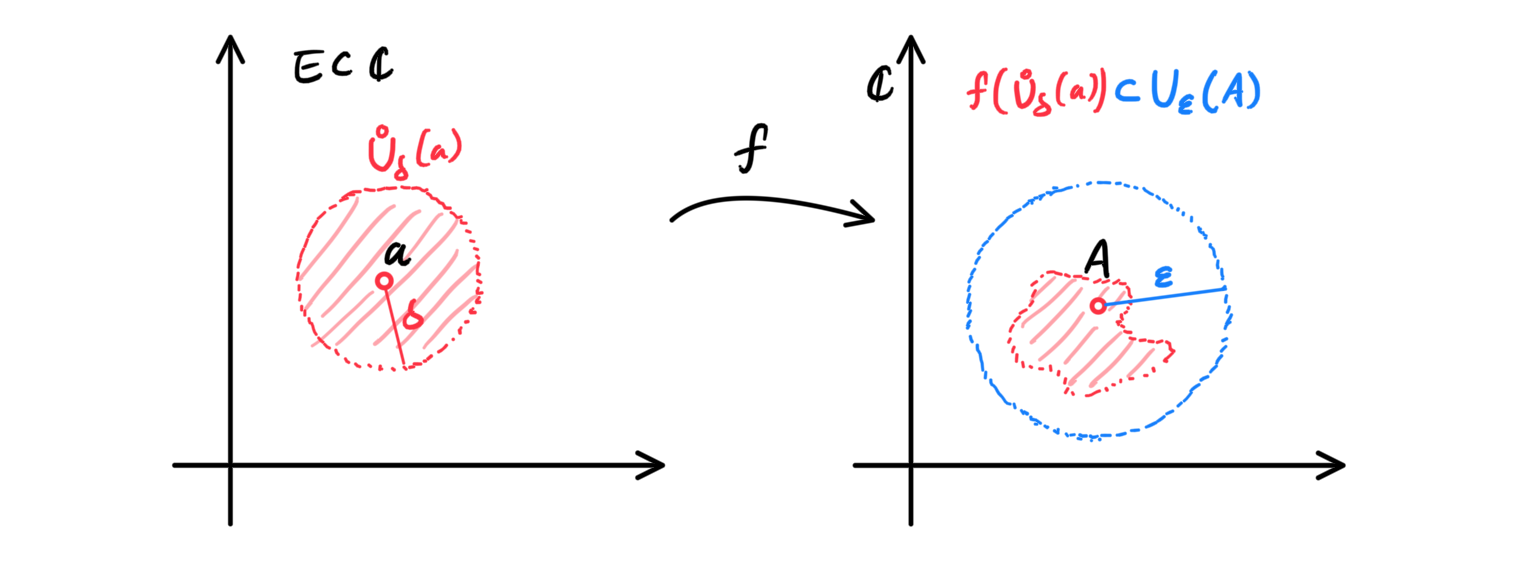
\includegraphics[scale=0.25]{img/Limit_of_Complex_Function.PNG}
      \end{center}
    \end{definition}

    \begin{definition}[Continuity of a Complex Function]
      A function $f: E \subset \mathbb{C} \longrightarrow \mathbb{C}$ is \textbf{continuous} at a point $z_0 \in E$ if for any neighborhood $U(f(z_0))$ there exists a neighborhood $U(z_0)$ such that its image is contained in $U(f(z_0))$. In short, 
      \[\lim_{z \longrightarrow z_0} f(z) = f(z_0)\]
      \begin{center}
        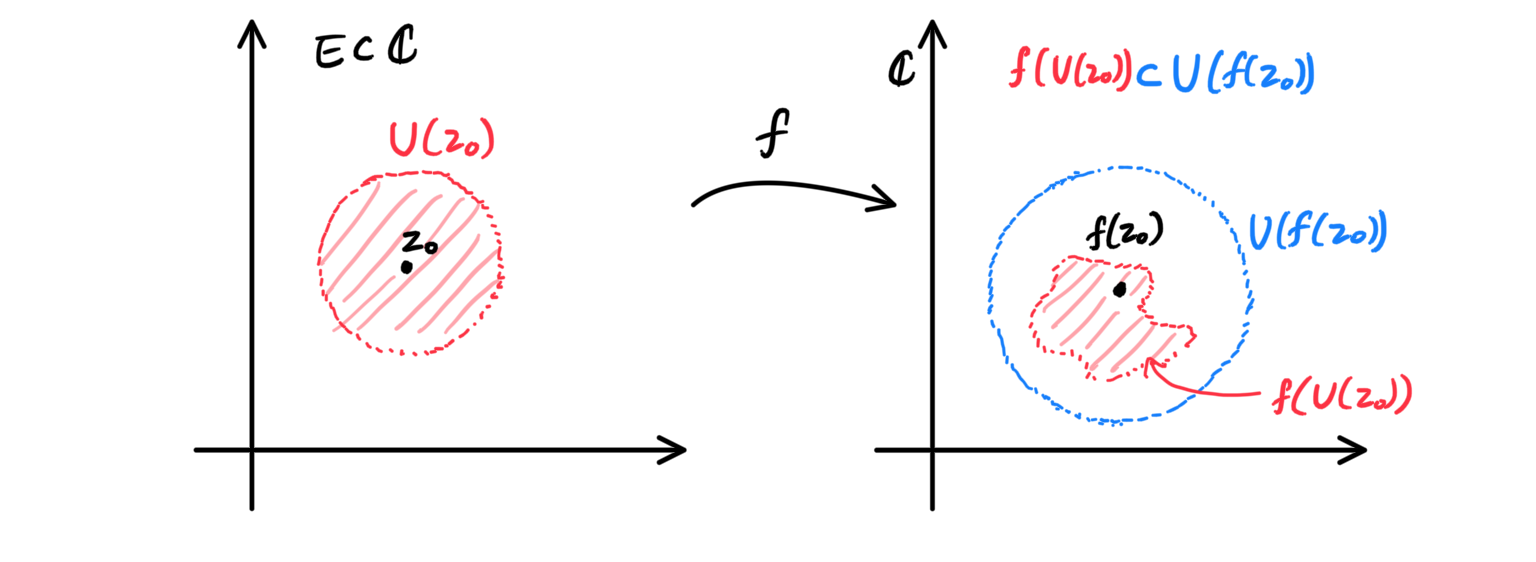
\includegraphics[scale=0.25]{img/Continuity_of_Complex_Function.PNG}
      \end{center}
    \end{definition}

    \begin{definition}[Differentiability of a Complex Function]
      The \textbf{derivative} of a function $f: E \subset \mathbb{C} \longrightarrow \mathbb{C}$ is defined
      \[f^\prime (z_0) = \lim_{z \rightarrow z_0} \frac{f(z) - f(z_0)}{z - z_0}\]
      if this limit exists. $f$ \textbf{differentiable} at $x_0$ means that a differential function 
      \[df(z_0): T_{z_0} \mathbb{C} \longrightarrow T_{f(z_0)} \mathbb{C}, \;\;\; h \mapsto df(z_0)(h)\]
      exists such that
      \[f(z) = f(z_0) + df(z_0)(h) + o(h)\]
      where $h = z - z_0$ is the increment of the argument. Just like the real case, it turns out that $df(z_0)(h) = f^\prime (z_0) h$, and 
      \[f(z) - f(z_0) = f^\prime(z_0) (z - z_0) + o(z - z_0)\]
      which elegantly weaves together the two concepts of differentiability and the derivative. 

      Visualizing this, we can see that for whatever function $f: \mathbb{C} \longrightarrow \mathbb{C}$ there is a linear function that transforms the entire space as such at $z_0$ (along with a given point $z_0 \in \mathbb{C}$), 
      \begin{center}
          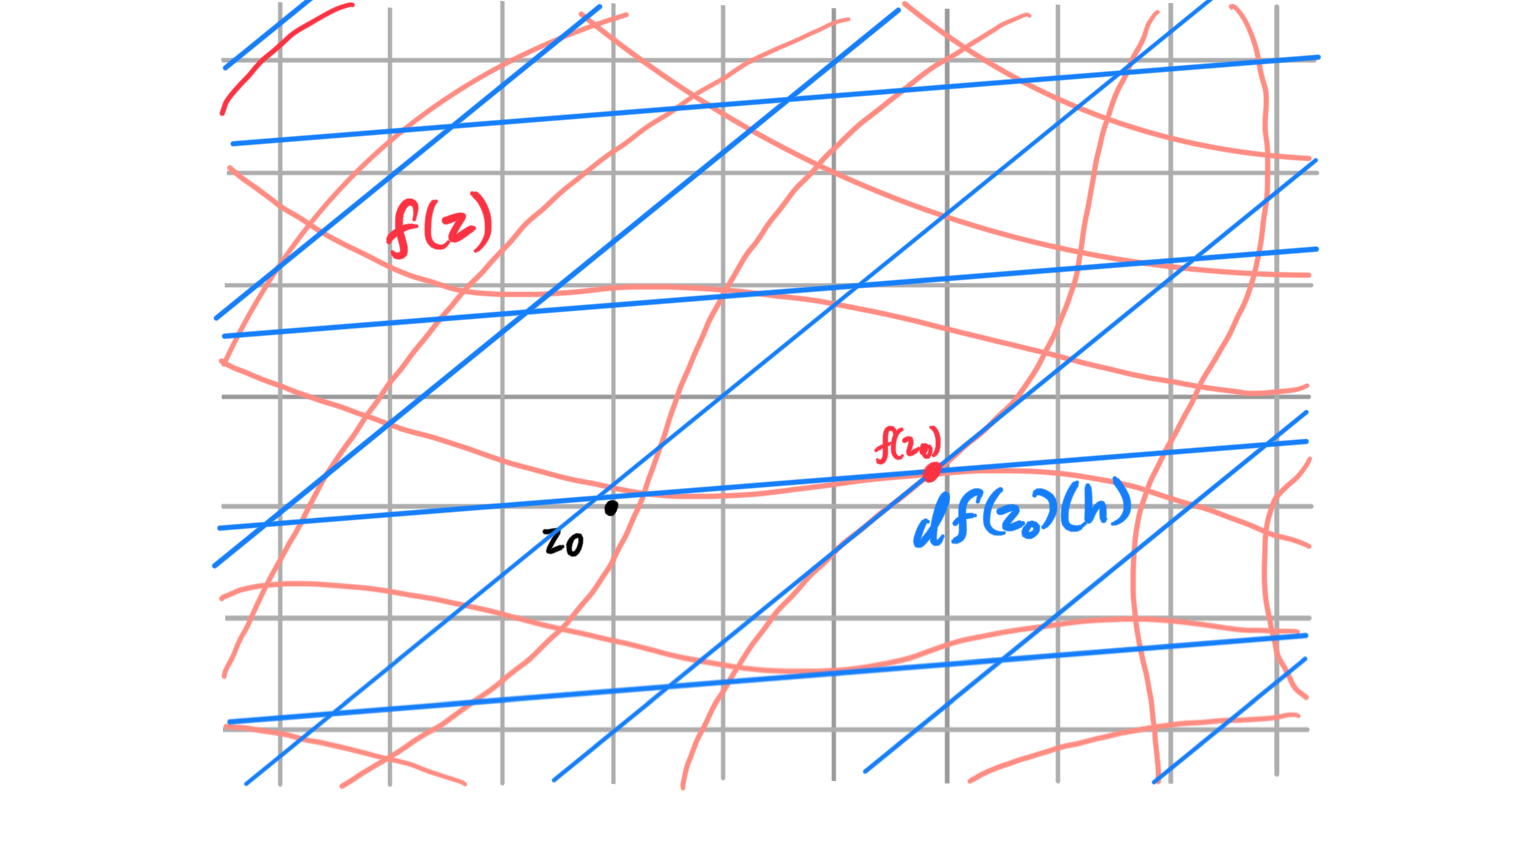
\includegraphics[scale=0.25]{img/Differential_of_Complex_Valued_Function.PNG}
      \end{center}
      The differential $df(z_0)$ at the point $z_0$ is a linear mapping that "best" approximates $f$, with an error of $o(h) = o(z - z_0)$. 
    \end{definition}

    \begin{lemma}[Arithmetic Properties of Differentiation over $\mathbb{C}$]
      If functions $f, g: E \subset \mathbb{C} \longrightarrow \mathbb{C}$ are differentiable at a point $z \in E$, then 
      \begin{enumerate}
        \item their sum is differentiable at $z$, and 
        \[d(f + g)(z) = df(z) + dg(z) \iff (f + g)^\prime (z) = (f^\prime + g^\prime)(z)\]
        \item their product is differentiable at $z$, and 
        \[d(f \cdot g) (z) = g(z) df(z) + f(z) dg(z) \iff (f \cdot g)^\prime (z) = f^\prime (z) g(z) + f(z) \cdot g^\prime (z)\]
        \item their quotient is differentiable at $z$ if $g(z) \neq 0$, and 
        \[d \bigg( \frac{f}{g}\bigg) (z) = \frac{g(z) df(z) - f(z) dg(z)}{g^2 (z)} \iff \bigg(\frac{f}{g}\bigg)^\prime (z) = \frac{f^\prime (z) g(z) - f(z) g^\prime (z)}{g^2 (z)}\]
      \end{enumerate}
      Just like the real case, the operation of taking the derivative is a linear operator. 
    \end{lemma}

    \begin{lemma}[Chain Rule for Composite Functions over $\mathbb{C}$]
      Let there be functions $f: E_1 \subset \mathbb{C} \longrightarrow \mathbb{C}$ differentiable at point $z \in E_1$ and $g: E_2 \subset \mathbb{C} \longrightarrow \mathbb{C}$ differentiable at point $w = f(z) \in E_2$, with respective differentials 
      \begin{align*}
          df(z) & : T_z \mathbb{C} \longrightarrow T_w \mathbb{C} \\
          dg(w) & : T_w \mathbb{C} \longrightarrow T_{g(w)} \mathbb{C}
      \end{align*}
      Then, the composite function $g \circ f: E_1 \longrightarrow \mathbb{C}$ is differentiable at $z$, and $d(g \circ f)(z): T_z \mathbb{C} \longrightarrow T_{g \circ f(z)} \mathbb{C}$ is
      \[d(g \circ f) (z) = dg(w) \circ df(z) \iff (g \circ f)^\prime (z) = g^\prime \big(f(z)\big) \circ f^\prime (z)\]
    \end{lemma}

    \subsubsection{Power Series Representation of a Function}
    \begin{definition}[Holomorphic Function]
      If function $f: E \subset \mathbb{C} \longrightarrow \mathbb{C}$ is (complex) differentiable at a point $z_0 \in E$, then $f$ is said to be \textbf{holomorphic at $z_0$}. 
    \end{definition}

    We recall the diagram that summarizes the conditions of differetiability and analyticity of a function $f$ over the field $\mathbb{R}$. 
    \begin{center}
    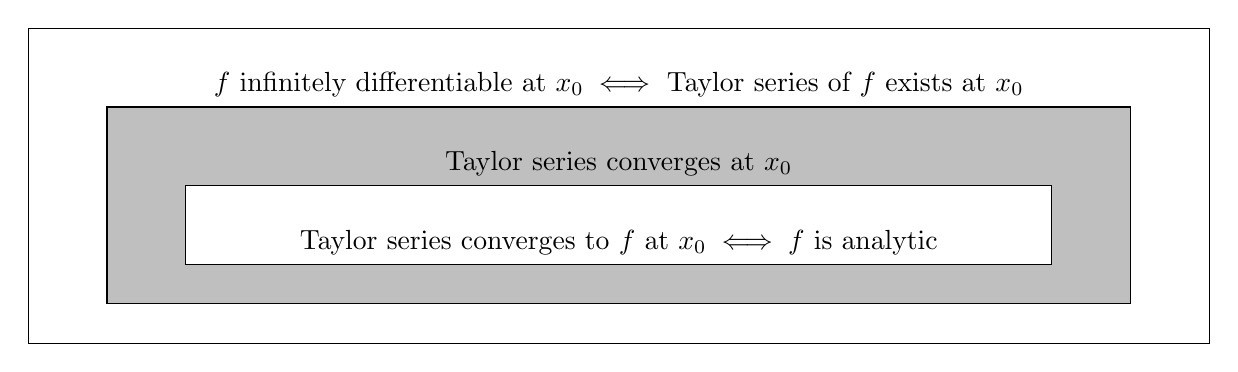
\begin{tikzpicture}
        \draw (-7.5,0) rectangle (7.5, 4);
        \draw[fill=lightgray] (-6.5, 0.5) rectangle (6.5, 3);
        \draw[fill=white] (-5.5, 1) rectangle (5.5, 2);
        \node[above] at (0, 1) {Taylor series converges to $f$ at $x_0 \iff f$ is analytic};
        \node[above] at (0, 2) {Taylor series converges at $x_0$};
        \node[above] at (0, 3) {$f$ infinitely differentiable at $x_0 \iff $ Taylor series of $f$ exists at $x_0$};
    \end{tikzpicture}
    \end{center}
    In the theory of functions of a complex variable we actually have a remarkable theorem that does not have an analogue for functions over $\mathbb{R}$. 

    \begin{theorem}[Analyticity of Differentiable Functions over $\mathbb{C}$]
    If a function $f: E \subset \mathbb{C} \longrightarrow \mathbb{C}$ is differentiable in a neighborhood of a point $z_0 \in E$, then it is analytic at that point. In other words, 
    \[f \text{ is holomorphic at } z_0 \implies f \text{ is analytic at } z_0\]
    This means that the conditions in the diagram above all are equivalent! Visually, 
    \begin{center}
    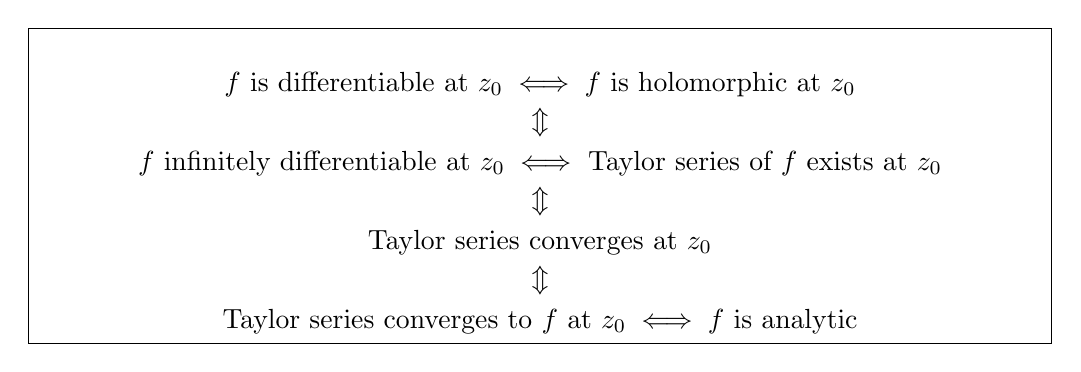
\begin{tikzpicture}
        \draw (-6.5,1) rectangle (6.5, 5); 
        \node[above] at (0,4) {$f$ is differentiable at $z_0 \iff f$ is holomorphic at $z_0$};
        \node at (0,3.8) {$\Updownarrow$};
        \node at (0,2.8) {$\Updownarrow$};
        \node at (0,1.8) {$\Updownarrow$};
        \node[above] at (0, 1) {Taylor series converges to $f$ at $z_0 \iff f$ is analytic};
        \node[above] at (0, 2) {Taylor series converges at $z_0$};
        \node[above] at (0, 3) {$f$ infinitely differentiable at $z_0 \iff $ Taylor series of $f$ exists at $z_0$};
    \end{tikzpicture}
    \end{center}
    This is certainly an amazing fact, since it then follows from the theorem that if a function $f(z)$ has one derivative $f^\prime (z)$ in a neighborhood of a point, it also has derivatives of all orders in that neighborhood. 
    \end{theorem}

    \subsubsection[Algebraic Closedness of the Field C]{Algebraic Closedness of the Field $\mathbb{C}$}

    \begin{definition}[Algebraically Closed Field]
      A field $\mathbb{F}$ is \textbf{algebraically closed} if every nonconstant polynomial in $\mathbb{F}[x]$ (the polynomial ring with coefficients in $\mathbb{F}$) has a root in $\mathbb{F}$. 
    \end{definition}

    \begin{theorem}[Fundamental Theorem of Algebra]
    $\mathbb{C}$ is algebraically closed. That is, every polynomial 
    \[P(z) \equiv c_0 + c_1 z + c_2 z^2 + \ldots + c_n z^n\]
    of degree $n\geq 1$ with complex coefficients $c_i \in \mathbb{C}$ ($i = 0, 1, \ldots, n$) has a root in $\mathbb{C}$. This immediately implies that every polynomial $P(z)$ admits a representation (unique up to the order of the factors) in the form 
    \[P(z) = c_n (z - z_1) (z - z_2) \ldots (z - z_n)\]
    where $z_1, \ldots, z_n \in \mathbb{C}$ not necessarily all distinct. 
    \end{theorem}

    We can also prove the interesting property about zeroes of polynomials in $\mathbb{R}[x]$. 

    \begin{corollary}[Complex Conjugate Roots of Real Polynomials]
    Given a polynomial with real coefficients
    \[P(z) \equiv a_0 + a_1 z + a_2 z^2 + \ldots + a_n z^n\]
    $P$, as we know, does not always have real roots (e.g. $P(x) = x^2 + 1$). However, we state that
    \[\text{if } P(z_0) = 0, \text{ then } P(\overline{z}_0) = 0\]
    Therefore, every polynomial $P$ with real coefficients can be expanded as a product of linear and quadratic polynomial with real coefficients. 
    \end{corollary}
    \begin{proof}
    We can see from the properties of complex numbers that
    \begin{align*}
        \overline{(z_1 + z_2)} & = \overline{z_1} + \overline{z_2} \\
        \overline{(z_1 \cdot z_2)} & = \overline{(r_1 e^{i \varphi_1} \cdot r_2 e^{i \varphi_2})} \\
        & = \overline{r_1 r_2 e^{i(\varphi_1 + \varphi_2)}} = r_1 r_2 e^{-i(\varphi_1 + \varphi_2)} \\
        & = r_1 e^{-i\varphi_1} \cdot r_2 e^{-i \varphi_2} = \overline{z}_1 \cdot \overline{z}_2
    \end{align*}
    Thus, if $P(z_0) = 0$, then 
    \[0 = \overline{P(z_0)} = \overline{a_0 + \ldots + a_n z_0^n} = \overline{a}_0 + \ldots + \overline{a}_n \overline{z}_0^n  = a_0 + \ldots + a_n \overline{z}_0^n = P(\overline{z}_0)\]
    and thus $P(\overline{z}_0) = 0$. 
    \end{proof}

  \subsection{Primitives}

    \begin{definition}[Primitive]
      A function $F(x)$ is a \textbf{primitive} of a function $f(x)$ on an interval if $F$ is differentiable on the interval and satisfies the equation 
      \[F^\prime (x) = f(x)\]
      or equivalently, if their respective differentials satisfy
      \[d F(x) = f(x) \,dx\]
    \end{definition}

    \begin{lemma}
      If $F_1(x)$ and $F_2 (x)$ are two primitives of $f(x)$ on the same interval, then the difference $(F_1 - F_2)(x)$ is constant on that interval. 
    \end{lemma}

  \begin{example}
  Both 
  \[F_1(x) \equiv \arctan{x} \text{ and } F_2(x) \equiv \arccot{\frac{1}{x}}\]
  are primitives of $f(x) = \frac{1}{1 + x^2}$. Indeed, we can see by direct calculation that in the domain $\mathbb{R} \setminus 0$, 
  \[F_1 (x) - F_2 (x) = \arctan{x} - \arccot{\frac{1}{x}} = \begin{cases}
  0, & x > 0 \\
  -\pi, & x < 0
  \end{cases}\]
  which is supported by the lemma. 
  \end{example}

    Notice how given a function $f(x)$, the operation of finding its differential, denoted with $d$, gives us a new function of $h$, called the differential 
    \[df(x)(h)\]
    Similarly, the operation of finding a primitive of function $f(x)$, denoted with the symbol $\int$, gives us a new function. 

    \begin{definition}[Indefinite Integration]
      The operation of finding a primitive of a certain function $f(x)$ is called \textbf{indefinite integration}, and the mathematical notation 
      \[\int f(x) \,dx\]
      is called the \textbf{indefinite integral of $f(x)$} on a given interval ($f$ called the \textbf{integrand} and $f(x)\,dx$ called the \textbf{differential form}). 
      \begin{enumerate}
        \item It immediately follows from the lemma that if $F(x)$ is any particular primitive of $f(x)$ on the interval, then on that interval 
        \[\int f(x) \,dx = F(x) + C\]
        \item If $F^\prime (x) = f(x)$ (that is, $F$ is a primitive of $f$ on some interval), then we have
        \[d \int f(x)\,dx = d F(x) = F^\prime (x) \,dx \]
        \item It also follows that 
        \[\int d F(x) = \int F^\prime (x)\,dx = F(x) + C\]
      \end{enumerate}
    \end{definition}

    \begin{theorem}[Basic Methods of Indefinite Integration]
    The definition of the indefinite integral has three basic properties that can be used to solve indefinite integrals. 
    \begin{enumerate}
      \item Linearity of the indefinite integral.
      \[\int \big( \alpha u(x) + \beta v(x)\big) \, dx = \alpha \int u(x)\,dx + \beta \int v(x)\,dx + C\]
      \item Integration by parts. 
      \[\int (u v)^\prime \,dx = \int u^\prime (x) v(x) \,dx + \int u(x) v^\prime (x) \,dx + C\]
      \item Change of Variable, or $U$-substitution. Given that $F^\prime (x) = f(x)$ on an interval $I_x$ and $\varphi: I_t \longrightarrow I_x$ is a $C^1$ mapping of interval $I_t$ into $I_x$, then
      \[\int (f \circ \varphi) (t) \varphi^\prime (t) \,dt = (F \circ \varphi)(t) + C\]
    \end{enumerate}
    \end{theorem}

